%
% --- inline annotations
%
\newcommand{\red}[1]{{\color{red}#1}}
\newcommand{\todo}[1]{{\color{red}#1}}
\newcommand{\TODO}[1]{\textbf{\color{red}[TODO: #1]}}
% --- disable by uncommenting  
% \renewcommand{\TODO}[1]{}
% \renewcommand{\todo}[1]{#1}

\usepackage{xcolor}
\usepackage{graphicx}
\usepackage{booktabs}
\usepackage{amsmath} 
\usepackage{amsfonts}
\usepackage{amssymb}
\usepackage{multirow} 
\usepackage{makecell}
\newcommand{\shline}{\Xhline{1.1pt}} % Adjust thickness as desired

\section{\ssm\ Architecture}
\label{sec:model}

The proposed architecture, \ssm, is composed of repeated identical blocks, each performing a sequence of information mixing steps across the different dimensions of the video signal: time, space, and channels; see Figure~\ref{fig:ssmvit}. The mixing over the time dimension is handled by gated linear recurrent units (LRUs), similar to the one introduced in~\citep{de2024griffinmixinggatedlinear} for language. Each spatial token is associated with an LRU that processes the tokens within the same \textit{temporal tube} over time, without mixing the information across temporal tubes. The LRUs share parameters over space, similar to a convolutional network. When applying this temporal mixing operation, the space dimension is transposed into the batch dimension.
The mixing over spatial and channel dimensions is handled by a standard ViT block, which first performs the spatial mixing through a self-attention operation, then the channel mixing by using an MLP. When performing the spatial and channel mixing, the time dimension is transposed into the batch dimension.

Empirically, we show that this factorization and choice of building blocks is more efficient for understanding temporal dynamics compared to video transformer approaches (e.g. ViViT~\citep{vivit}) or pure SSM models. By applying self-attention over the spatial dimensions, we allow all tokens to attend to all the other tokens in  parallel, without having to commit to a particular order (unlike in VideoMamba). We employ strong transformer blocks from ViTs for this operation, including their Imagenet pre-trained weights. The recurrence of the temporal processing enables efficient frame-by-frame inference over long videos, with constant memory footprint and causal operation. 

\subsection{Background on LRUs}

Linear Recurrent Units (LRUs)~\citep{orvieto2023resurrecting}, similar to SSMs, belong to the family of linear recurrent architectures and have been shown to be competitive with Transformers on language tasks~\citep{de2024griffinmixinggatedlinear,gu2023mamba}. One potential interpretation of the success of these models, as outlined in~\citep{orvieto2023resurrecting}, is that by sacrificing the nonlinear recurrence typical of a recurrent model, we can improve the scalability and controllability of the system. Specifically, the linearity allows the recurrent matrix to be diagonalised through eigenvalue decomposition and absorbing the (dense) eigenvectors matrix into the neighbouring layers. This gives direct access to the eigenvalues of the Jacobian of the transfer function characterising the system. By initialising these eigenvalues within the unit circle, we have guaranteed stability of the system, bypassing issues like vanishing or exploding gradients. In addition, through the specific initialisation range of the eigenvalues within [0, 1] we can control how quickly the information vanishes, with eigenvalues close to 1 promoting longer-term memory. However, using only linear recurrence can greatly limit the expressivity of the layer. In ~\cite{orvieto2023universality}, the authors show that by using these layers within a typical transformer structure that alternates linear recurrences with point-wise nonlinearities (\eg the MLP block), the overall architecture can be shown to be a universal approximator of finite sequence-to-sequence maps.     

\subsection{Gated LRUs for Video}
We adopt the gated variant of the LRU~\citep{de2024griffinmixinggatedlinear} to design our proposed block for video modelling. 

Let $X\in[0, 1]^{T \times H \times W \times 3}$ be an RGB video with $T$ frames and $H \times W$ pixels. The video frames are split into $N$ non-overlapping patches $p_t^k$ of size $n\times n \times 3$, with $t\in\{1,T\}$ and $k\in\{1, N\}$. Let $x_t^k$ be the tokens obtained after the linear projection of the patches and the addition of the spatial positional encoding, with token size $1\times 1 \times d$, where $d$ is the token feature dimension. Each LRU operates over a \textit{temporal tube} $\{x_t^k|t=\overline{1,T}\}$, following the equations below (we drop the $k$ spatial index for clarity):    


\begin{eqnarray}
i_t & = & \sigma(W_x x_t + b_x), \quad\,\,\, \textcolor{gray}{\text{\emph{ input gate}}} \label{eq:input_gate}\\
r_t &=& \sigma\left(W_\lambda x_t + b_\lambda\right), \quad \textcolor{gray}{\text{ \emph{recurrence gate}}} \label{eq:recurrent_gate} \\
\lambda_t &=& \sigma(\lambda)^{\text{C} \cdot r_t}, \label{eq:a_rglru} \\
h_{t} &=& \lambda_t \odot h_{t-1} + \sqrt{1-\lambda_t^2} \odot (i_t \odot x_t).
\label{eq:RG_LRU}
\end{eqnarray}


\noindent where $h_t \in \mathbb{R}^d$ is the state of the LRU, $\lambda_t\in \mathbb{R}^d$ is a vector containing the eigenvalues of the (diagonal) recurrence matrix\footnote{Similar to \cite{de2024griffinmixinggatedlinear}, we implement the recurrence weights $\lambda_t$ as ${\exp(-C\cdot \text{softplus}(\lambda)\cdot r_t)}$, which is mathematically equivalent but numerically more stable.}, $i_t \in \mathbb{R}^d$ is the input gate controlling whether $x_t\in \mathbb{R}^d$ is integrated within the state $h_t$ of the LRU or not, and $r_t\in\mathbb{R}^d$ is the recurrence gate.
The weights and biases of the LRU ($W_x\in \mathbb{R}^{d \times d}$, $W_\lambda \in \mathbb{R}^{d \times d}$, $b_x \in \mathbb{R}^d$, $b_\lambda \in \mathbb{R}^d$) are initialized using LeCun init~\cite{LeCun2012}. 

The (learnable) recurrence weights $\lambda$ are passed through a sigmoid function to ensure they are between $0$ and $1$, and are initialised such that $\sigma(\lambda)$ is sampled uniformly in $[\lambda_{\min}, \lambda_{\max}]$. These recurrent weights are raised to the power $\text{C} \cdot r_t$, which effectively acts as a \emph{gate} controlled by $r_t$ given in equation~\eqref{eq:recurrent_gate}. $r_t$ is defined as a linear projection, with parameters $W_\lambda$ and $b_\lambda$, followed by a sigmoid function to ensure again the range $[0,1]$. By raising element-wise $\sigma(\lambda)$ to $r_t$, the effective recurrence weight at some position $j$ can change between the $j$-th entry of $\sigma(\lambda)$ when the corresponding gate entry is $1$ and $1$ when the gate entry is 0. 

The additional constant coefficient $\text{C}\in \mathbb{R}$, typically set to 8 as in~\cite{de2024griffinmixinggatedlinear}, increases the range to be between $\sigma(\lambda)^\text{C}$ to $1$, providing additional flexibility. \Eg if $\sigma(\lambda)$ is $0.9$ and we set $\text{C}=8$, we extend the range from $[0.9, 1]$ to $[0.43, 1]$. More importantly, we change the learning dynamics (\eg gradient norms) and resolution we have over the range during learning. Specifically, for $x_t$ in some fixed interval and similar magnitude $W_\lambda$, as it is the case at initialisation, a higher value of $\text{C}$ implies $\lambda_t$ will concentrate more towards the edges of the range. Note also that this is the dynamic range in which the recurrent weights can vary during inference as a function of the input tokens. 

In~\cite{de2024griffinmixinggatedlinear}, the authors found that setting $\lambda_{\min}=0.9$ and $\lambda_{\max}=0.999$ leads to the best results. An eigenvalue of $0.9$ implies that it will take at least $10$ time steps for the information to decay to roughly $35\%$ of its magnitude, while for an eigenvalue of $0.999$ it will take $1000$ time steps to decay by the same amount. When using the same range for video modelling, we observed that the eigenvalues are pushed significantly towards $\lambda_{\min}$ during training, with a small number of eigenvalues becoming smaller than $\lambda_{\min}$; see Figure~\ref{fig:eigs}. We experimented with extending the range and obtained better results with $\lambda_{\min}=0.6$. This leads to faster decay of information initially and might reflect the importance for videos of having enough recurrent units focused on short term information, in order to disentangle fast changing dynamics from slow ones.

\begin{figure}[h]
\centering
    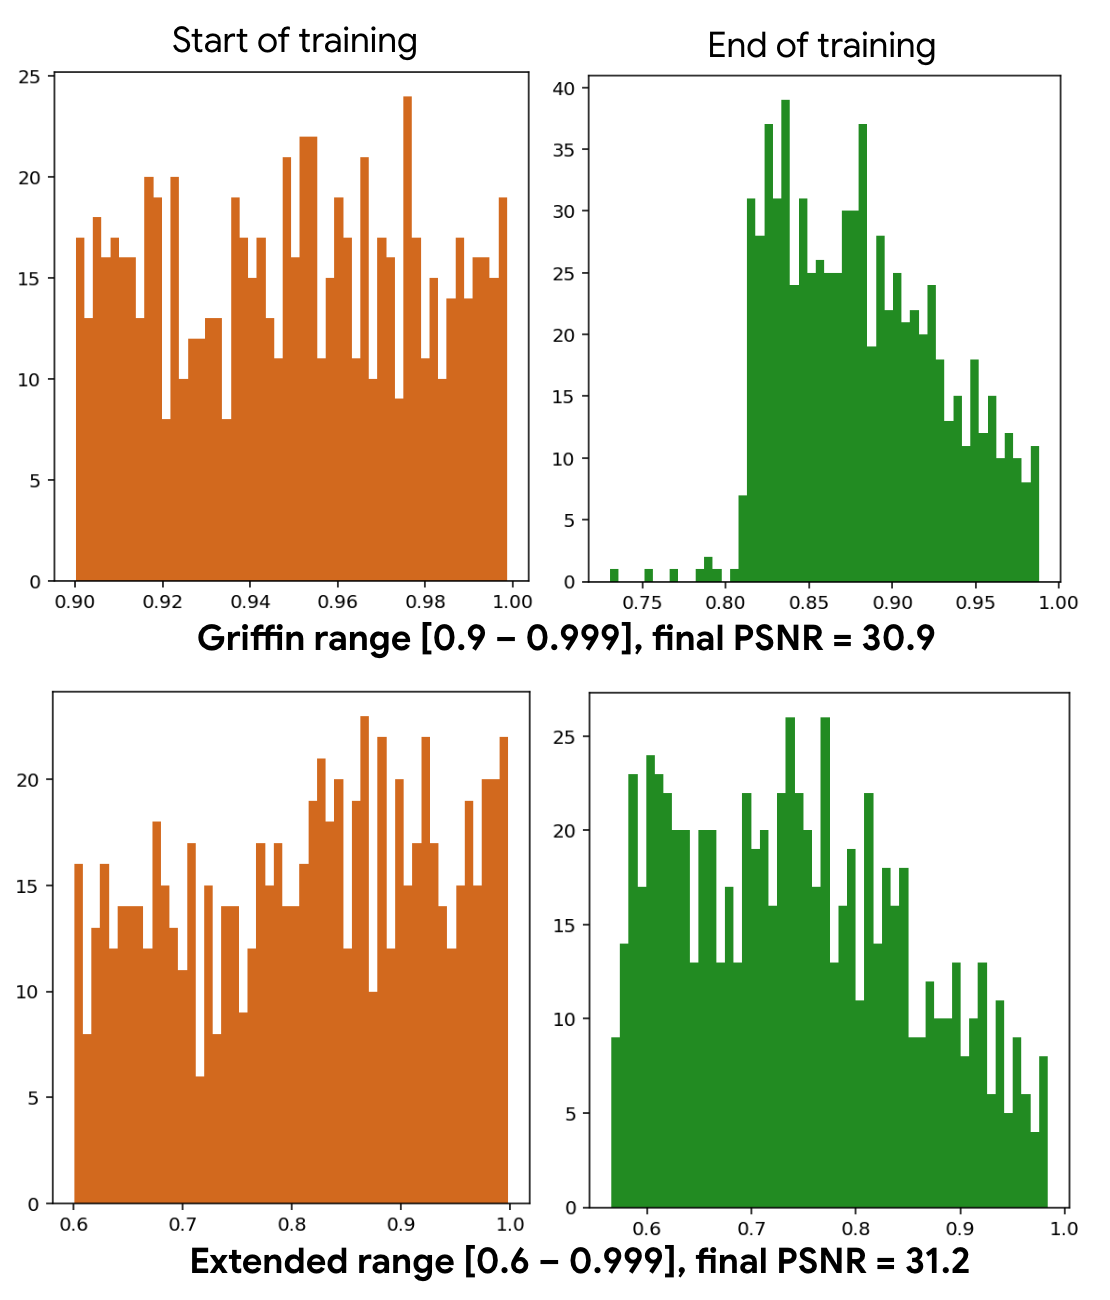
\includegraphics[width=.8\linewidth]{img/eigs.png}
\caption{Distribution of the eigenvalues of the recurrent matrix at the beginning and end of training on long video memorisation task (see subsection~\ref{sec:longtask}) for different initialisation ranges.}
\label{fig:eigs}
\end{figure}

Finally, note that when diagonalising the recurrence matrix, the eigenvalues $\lambda$ could, in theory, have complex values. We conducted experiments using complex eigenvalues, but we did not see improvements compared to using only real eigenvalues. The same observation was made in ~\cite{de2024griffinmixinggatedlinear,gu2023mamba} as well. 

\begin{figure*}[t!]
\centering
\begin{subfigure}{0.48\textwidth}
    \centering
    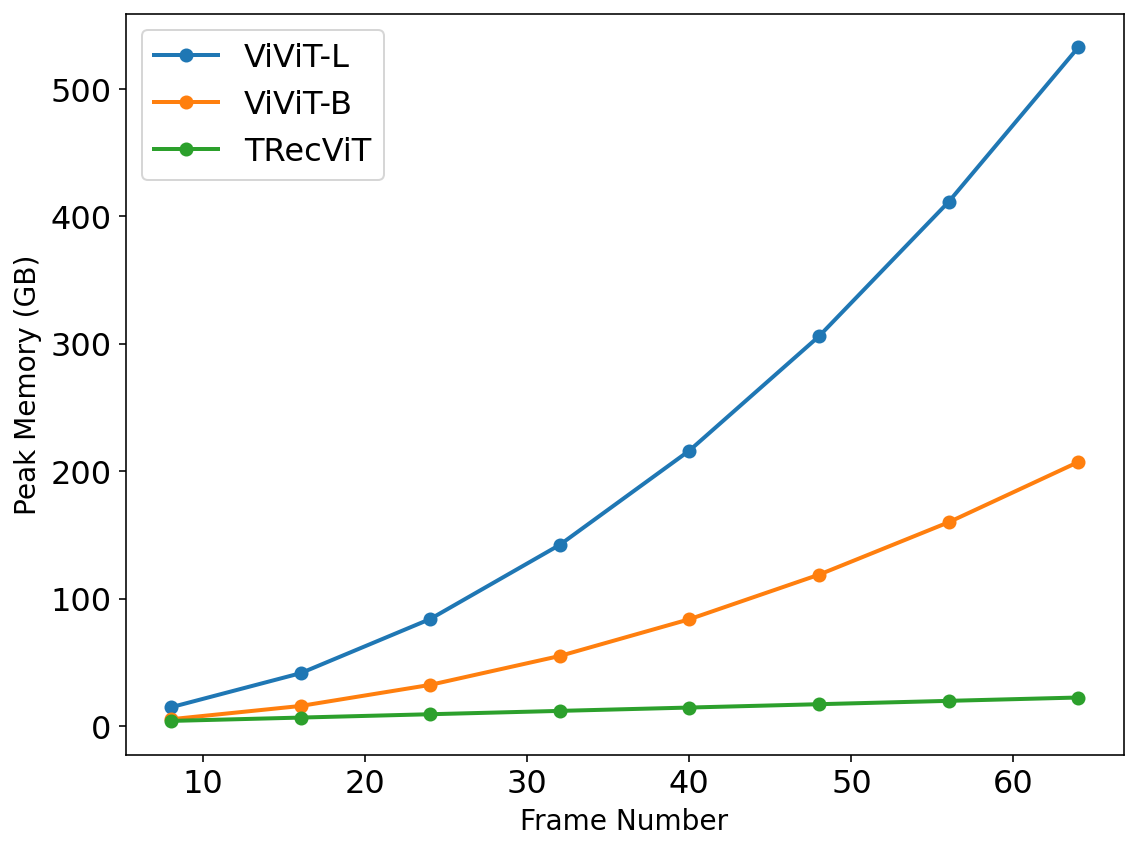
\includegraphics[width=.9\textwidth]{img/memory.png}
    \caption{Memory comparison}
\end{subfigure}%
\hfill
\begin{subfigure}{0.48\textwidth}
    \centering
    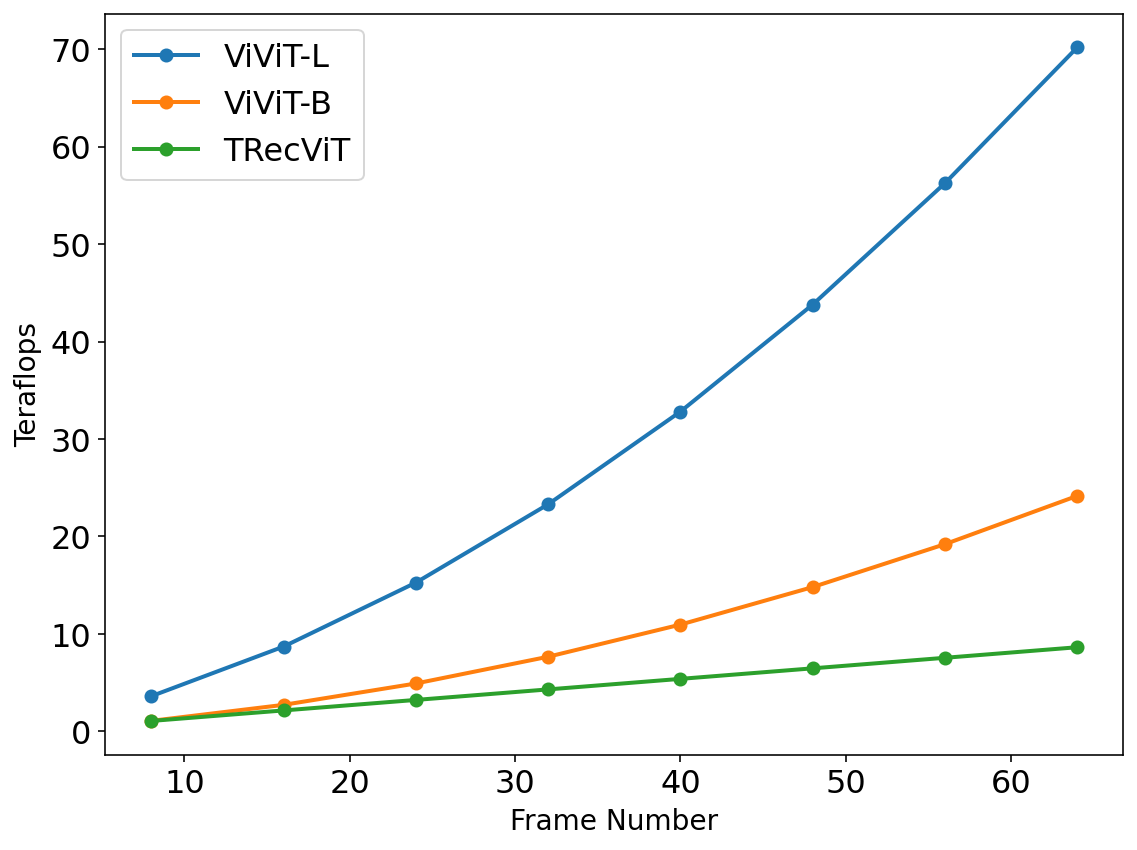
\includegraphics[width=.9\textwidth]{img/flops.png} 
    \caption{FLOPs comparison}
\end{subfigure}
\caption{Our model demonstrates increasingly greater memory and compute savings compared to ViViT baselines as the number of frames increases. For clarity, \ssm's peak memory (left figure) goes from about 4G for 8 frames to 22.4G for 64 frames, but this increase is dwarfed by ViViT's increase, hence \ssm\ line appears almost horizontal
}
\label{fig:memory}
\end{figure*}

\subsection{Video block based on gated LRU}

We use the gated LRU in a similar block structure as the one employed in~\cite{de2024griffinmixinggatedlinear}, see Figure~\ref{fig:ssmvit}b. 
Given a 1D input (temporal tube), the block first applies a normalisation layer, then the signal is routed on two different paths. On the first one, it gets linearly projected to same dimensionality $d$  and then the \emph{GeLU} activation is applied. On the other path, the signal is also linearly projected to the same dimensionality $d$, then we apply a 1D convolution followed by the gated LRU described in equation~\eqref{eq:RG_LRU}. The output of the LRU and the GeLU branch are element-wise multiplied and then linearly projected to the same dimension $d$. Note that, in line with~\cite{de2024griffinmixinggatedlinear}, we use a separable convolution, which allows mixing information only over time, not over channels. We sweep the width of the convolutional kernel and find that a window of 2 is enough compared to~\cite{de2024griffinmixinggatedlinear} which used 4. Also, different from ~\cite{de2024griffinmixinggatedlinear}, we do not use an MLP block after the LRU for feature mixing. We apply the MLP after the self-attention block, as done in ViT. 

Given the diagonal form of the recurrence, on device, the gated LRU computations are memory-bound, \ie the data transfer takes longer than the actual computations done on that data. Similar to~\cite{de2024griffinmixinggatedlinear} we use a specialised \emph{Pallas}~\cite{jax2018github} kernel that minimizes the number of bytes that need to be moved between HBM and VMEM (the Vector Processing Unit's cache). The parameters added by the linear projections within the block, as well as the parameters of the convolution and the LRU, are learned.

% \todo{explain how many parameters we are adding with the LRU}

\section{Training \ssm}
\label{sec:training}

The proposed architecture can be trained in a supervised or self-supervised regime. Given a tokenised video input, the output of \ssm\ will have the same dimension and shape as the input, meaning that we can easily recover the spatio-temporal structure of the input video, which can be useful for dense tasks like pixel reconstruction, depth estimation, or point tracking. At inference time, the architecture can be applied over all the video frames at once, or frame-by-frame by carrying over the state of the LRUs. Depending on the task, one can choose to keep all the outputs from all time-steps to make a prediction (similar to ViViT), or just the outputs from the last step, given that the LRU integrates the previous history in its state. In our experiments, we use mainly the former for fairer comparison with ViViT, but we also experiment with the latter to analyse LRU's capability of remembering over a very long context; see subsection~\ref{sec:longtask}.   

\subsection{Self-supervised pre-training}

Given the factorised nature of the proposed architecture and the redundancy present in the video signal, it comes natural to apply masked auto-encoding to enable self-supervised pre-training from scratch on large-scale unlabelled datasets. 

We follow the same recipe as in the original VideoMAE paper~\citep{tong2022videomae}. Specifically, we use tube masking where a 2D random mask is generated and repeated for all the frames in the video. For our architecture, this is equivalent to dropping temporal LRUs. The training objective is simply L$_2$ reconstruction error of the entire frames. We sweep the value of the masking ratio and we find that 0.90 leads to best performance on downstream tasks. When using the pre-trained representations for downstream tasks, we keep all the tokens of the video and we add a decoder or readout head that is fine-tuned for the respective tasks.


\subsection{Memory footprint and FLOPs}
We compare the memory footprint and the number of FLOPs of \ssm\ against ViViT baselines, see Figure~\ref{fig:memory}. 
The profiling results are obtained by cost and memory analysis of lowered Jax HLO on CPU backend to be aligned with the theoretical numbers~\cite{jaxstatix}. We consider as input a video of size $224\times224$ and we vary the length of the video to analyse the savings provided by our architecture as the length of the video increases. Although in number of parameters for \ssm\ is in between ViViT-B and ViViT-L (90M $>$ 109M $>$ 320M), the peak memory and number of flops for \ssm\ are significantly lower as the number of frames increases, \eg at 32 frames (the number of frames typically used in video classification experiments), \ssm's peak memory is $\sim$12$\times$ smaller than that of ViViT-L and the FLOPs count is $5\times$ lower. When going to 64 frames, the peak memory is $\sim$24$\times$ smaller and FLOPs count is $8\times$ lower. 